\chapter{Regroupement Modulaire}

Dans la \autoref{fig:25-regroupement_modulaire}, nous pouvons identifier les multiples parties composant notre application.

\begin{figure}[h]
    \centering
    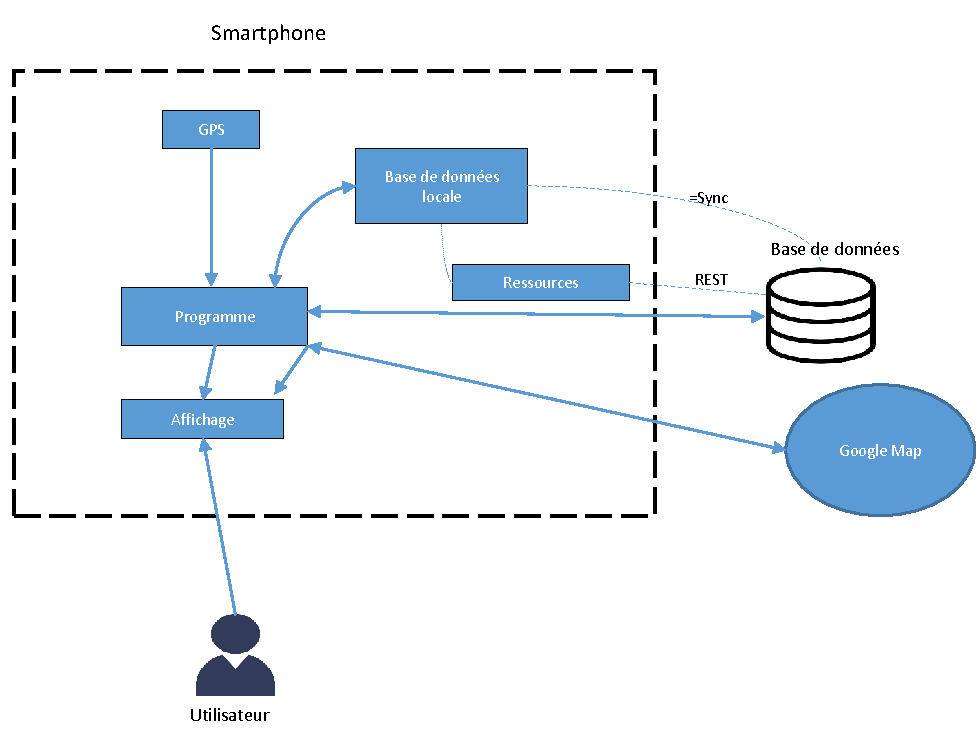
\includegraphics[keepaspectratio, width=2\textwidth/2, height=2\textheight/5]{ima/regroupement_modulaire}
    \caption{Schéma fonctionnel de notre projet.}
    \label{fig:25-regroupement_modulaire}
\end{figure}

\section{GPS}
GhostRun a besoin de récupérer le trajet de l'utilisateur, et pour pouvoir connaitre l'évolution de la position de l'utilisateur
dans le but de l'afficher lors d'un futur trajet. De ce fait l'intervalle de temps entre 2 relevé de position doit être faible.
(de l'ordre de la seconde.)
Le fait de connaitre la position de l'utilisateur à cette fréquence nos permet d'afficher un fantôme qui se déplace de manière continue dans le temps,
mais aussi de connaitre l'évolution de la vitesse au fur et à mesure du trajet.
% Expliquer ce que c'est, ce pourquoi l'appli s'en sert et à quelle fréquence, etc..

\section{Base de données}

\section{Google Maps}

\section{Resources externes}

\section{Affichage}
